\renewcommand{\figurename}{}
\mychapter{R3.ROM16 Ingénierie de la téléphonie sur IP (22h30)}{cap:r3rom16} 
\lhead{R3.ROM16 Ingénierie de la téléphonie sur IP (22h30)}

\vspace*{0.2cm}%
      \large
      \href{}{\color{black}Enseignant\\M. Angel Abénia}\\%
      \normalsize
\vspace*{0.5cm}%

Ce module accès sur la ToIP \textit{Téléphonie sur IP} fait suite aux enseignements reçus en première année sur VoIP \textit{Voix sur IP}. Nous y avons revu la numérisation de la voix, pour y ajouter les technologies logicielles et réseaux permettant son transport et leur mise en place en entreprise.
\\ \\
Ainsi, nous y avons étudié les codecs, le framing et la VAD pour basculer la donnée analogique et continue qu'est la voix dans le monde du numérique. Nous y avons abordé son transport sur le réseau avec les protocoles RTP et RTCP. Pour finaliser notre apprentissage par le montage d'une infrastructure ToIP afin d'analyser la signalitique utilisée pour l'émission et la gestion des appels en entreprise de nos jours.

\section{Capture de la voix vers le numérique}
% trois types de codecs
% codecs G721, G711
% pas précisé codec pour codeur décodeur

La voix est une donnée analogique, c'est un flux constant d'informations matérialisé par la vibration de l'air, retranscrit dans nos tympans et interprêté par notre cerveau. Nous arrivons à la numériser, de la passer du monde analogique (phénomène physique du son) à celui du numérique (de l'informatique, avec des nombres).
\\ \\
Cette conversion analogique-numérique débute par l'échantillonnage de la voix : on place une membrane pour reproduire artifitionnellement nos tympans dans un micro, pour poser une valeur numérique sur la vibration que la membrane reçoit.

% \begin{figure}[H]
\begin{figure}[hp]
    \centering
    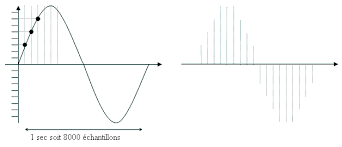
\includegraphics[width=\textwidth - \textwidth / 5]{ressources/r3rom16/00.png}
    \caption{La vibration reçue s'apparente à une fréquence, l'échantilloneur pose 8000 points par secondes dessus pour avoir une voix échantillonnée à 8 KHz et le codeur définit le nombre d'étages que ces points peuvent prendre en bits multiples de 2}
    \label{fig:echantillonnage}
\end{figure}

\noindent En jouant sur ces paramètres, on peut retrouver une voix plus ou moins fidèle à l'analogique car plus d'échantillons seront pris pour caractériser la voix (échantillonnage), ou plus ceux-ci pourront être variés car plus d'étages (codage). Une compression est souvent présente, car chaque étage correspond à une valeur chiffrée multiple de 2 (2 bits, 4 bits...) et l'échantillonnage définira la fréquence à laquelle on souhaitera générer des nombres avec ces valeurs (pouvant vite prendre de la place).
\\ \\
La compression se retrouve extrêmement utile pour stocker la voix et la transmettre sur le réseau. Les ensembles échantillonnage, codage et compression ont été normalisés pour que les téléphones et autres appareils audio puissent enregistrer et rejouer les mêmes enregistrements. Ainsi sont nés les codecs audio.
\\ \\
Ceux-ci sont extrêmement importants en réseau car définissent la quantité de données envoyés (rappel, elles prennent de la place). Les deux codecs les plus utilisées sont le G 711 et le G 729. Le G 711 propose 8 KHz d'échantillonnage sur 8 bits avec 0,125 ms de temps de compression : 64 kbits/s seront envoyés sur le réseau (prendra davantage de bande passante que le G 711 avec ses 8 kbits/s).
\\ \\
Nous avons étudié les codecs, le framing, la VAD impactant le stockage et le transport de la voix sur les réseaux. Ainsi, nous pourrons efficacement comprendre, dimmensionner et corriger des problèmes impactant la téléphonie sur IP d'une entreprise.

\section{Transporter une information continue sur un réseau}
% problème des applications temps réels
% RTCP, RTP

Le transport de la voix sur le réseau impose des problématiques non rencontrés auparavant par les flux de données (téléchargement de fichiers, vidéo à la demande...). Une conversation orale ne peut se permettre de perdre un bout de l'information, encore moins de la redemander à chaque fois, que l'on vérifie à chaque fois que l'information soit bien arrivée, ou que les morceaux de la phrase n'arrivent pas en même temps.
\\ \\
Pour compenser ces problèmes instaurés par l'utilisation de réseaux à commutation de paquets comme IP, un système de priorisation été mis en place pour ceux l'utilisant : la QoS \textit{Qualité de Service}. Ainsi, les paquets comportant de la voix seront privilégiés en étant routés ou commutés plus vites que les autres (pour éviter les latences, les gigues...).
\\ \\
Des protocoles de couche 4 ont été étudiés pour le transport de la voix dit \textit{"temps réel"}, et toujours largement utilisés : RTP et RTCP. Nous comprennons désormais les téchnologies permettant de transmettre la voix sur le réseau.

\section{Comment les appels sont passés en ToIP}
% signalisation SIP

Les signalisation téléphoniques sur la ToIP ont été standardisés afin de pouvoir initier, manipuler ou raccrocher un appel de la même manière sur la plupart des appareils.
\\ \\
Pour cela, les terminaux de la ToIP utilisent le protocole SIP \textit{Protocole d'Initiation de Sessions}. Les terminaux communiquent avec un serveur dédié à la signalitique et la gestion des communication (Provider SIP) qui se chargera d'envoyer une trame pour effectuer une action.

\begin{figure}[H]
      \centering
      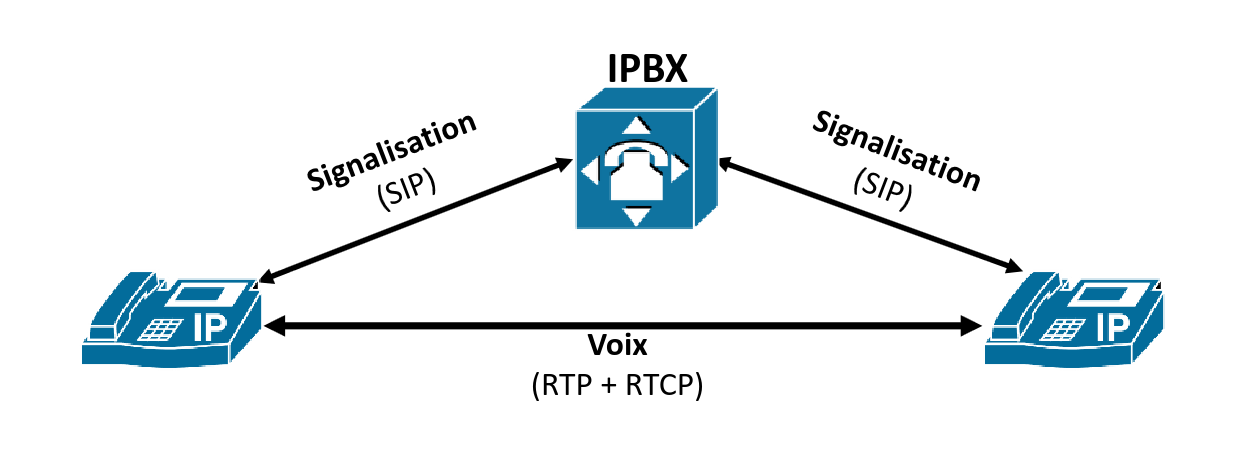
\includegraphics[width=\textwidth - \textwidth / 3]{ressources/r3rom16/01.png}
      \caption{Exemple simplifié de signalisation entre deux appareils utilisant le même Provider SIP.}
      \label{fig:echantillonnage}
\end{figure}

\noindent Nous avons ainsi analysé et étudié le trafic SIP généré pour différentes actions téléphoniques avec l'analyseur de trâmes Wireshark. Nous comprennons désormais les notions utilisées pour les communications d'entreprise basées sur de la ToIP.